\documentclass{ximera}
\author{Wim Obbels \and Bart Snapp}
\license{CC: 0}

\title{Basic Answer Types}

\begin{document}
\begin{abstract}
    A simple Ximera activity.
\end{abstract}
\maketitle

Perhaps the most natural setting for Ximera content is that of a
\textit{worksheet}. This is some document that may contain discussion as well
as questions that check understanding.

Ximera comes pre-equipped with many environments. We use
\verb|\begin{definition}| for definitions and \verb|\begin{question}| for
questions. Since Ximera provides immediate feedback, we suggest following
definitions like this one by a quick question. If you are ever curious about
the source code, you can visit this source at

\begin{center}

    \url{https://github.com/ximeraProject/ximeraFirstSteps/basics/basicAnswerTypes.tex}
\end{center}

or by appending \verb|.tex| to the URl of this page online. Here's an example:

\begin{definition}
    The \textbf{absolute value} of a real number $a$, denoted by $|a|$, is
    \[
        |a| = \begin{cases}
            a  & \text{if $a \geq 0$} \\
            -a & \text{if $a<0$.}
        \end{cases}
    \]
\end{definition}
Now students can check their understanding:
\begin{question}
    \begin{enumerate}
        \item $|2-5| = \answer{3}$
        \item $|5-2| = \answer{3}$
        \item $|5-\sqrt{2}| = \answer{3.58578643763}$
        \item $|5-\sqrt{2}| = \answer{5-\sqrt{2}}$
    \end{enumerate}
\end{question}

After that, you might want to have some exercises:

\begin{exercise}
    Let $x$ be the number of people
    out of $100$ that LOVE Ximera.

    Find the value of $x$.
    \[
        x = \answer{100}
    \]
\end{exercise}

Maybe you want a problem with one or more parts,

\begin{exercise}
    Ximera is so awesome because it feels like:
    \begin{multipleChoice}
        \choice{Doing taxes}
        \choice{Writing a book by hand}
        \choice[correct]{A walk in the park with free ice cream} 
        \choice{Solving a puzzle blindfolded}
    \end{multipleChoice}
    Why is Ximera the best thing since the chalkboard?
    \begin{selectAll}
        \choice[correct]{It turns \LaTeX\ into online materials}
        \choice[correct]{It boosts student engagement}
        \choice{It makes coffee and hugs you}
        \choice[correct]{Its Open-source and free}
    \end{selectAll}
\end{exercise}
\end{exercise}

Finally we can include pictures using \verb|includegraphics| like this

Here we see an included a JPEG and a PNG:

\begin{verbatim}
\begin{image}
  
\includegraphics[width=.3\textwidth]{missionPatch.jpg}\qquad
  \includegraphics[width=3in]{}
\end{image}
\end{verbatim}
In the code above, the command image is just a Ximera provided wrapper
that can be redefined for printing.
\begin{image}
  
\includegraphics[width=5in]{missionPatch.jpg}%\qquad
  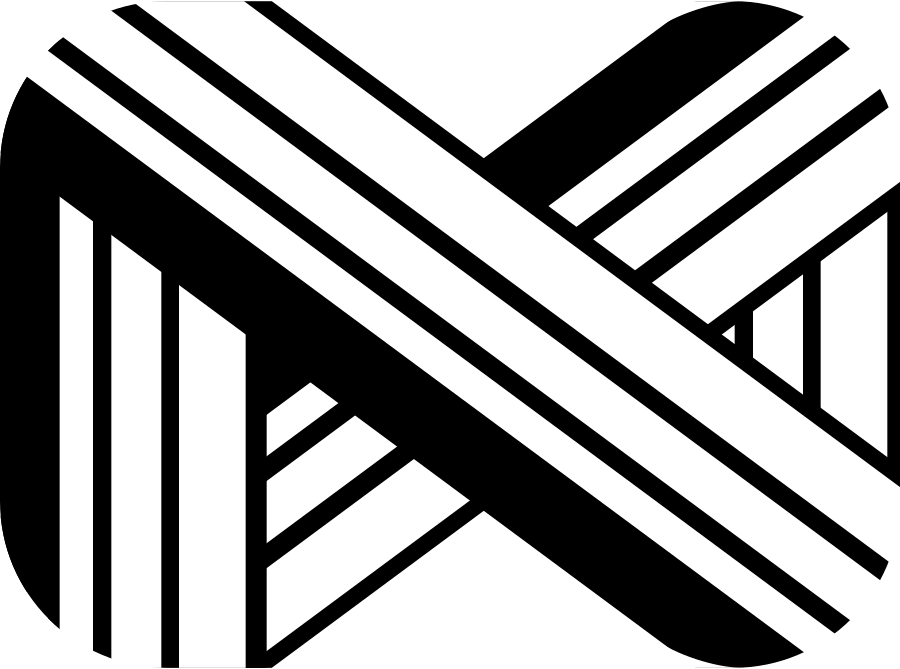
\includegraphics[width=.3\textwidth]{mx.png}
\end{image}
Here we have a pdf
\begin{center}
  
\includegraphics{llama.pdf}
\end{center}

\end{document}